%!TEX root = ../../main.tex
\section{Experimental methods}
\label{sec:Experimental methods}
This section describe the experimental details for two experiments comparing the efficacy of various radioprotectant compounds. The first of these experiments was carried out in 2014 whereas the second was carried out in 2015.

\subsection{Sample preparation}
\label{sub:Sample preparation}
\textcolor{red}{
    \begin{myenumerate}
        \item \hypertarget{todo:Need info from Ed}{\textbf{TODO:} Get following info from Ed:}
        \begin{itemize}
            \item Where was GI purchased? (Hampton Research?)
            \item what form was GI in when purchased? (jeffries et al. study said crystalline suspension?)
            \item What was the buffer composition that GI was dialysed against?
            \item What temperature was dialysed at? ($277\ K$)
            \item How long was it dialysed?
            \item pH was 7.0? (I think it was)
            \item where was the extinction coefficient information obtained? what was the extinction coefficient? and at what wavelength was this tested?
            \item Final concentration used in the experiment was? (I think it's $1 mg/ml$)
        \end{itemize}
    \end{myenumerate}
}
Crystalline glucose isomerase (GI) used in both experiments was purchased in tetrameric form (1552 residues, 172 kDa) from \textcolor{red}{...}.

\subsubsection{Experiment 1}
\label{subs:Experiment 1 - sample prep}
Radioprotectants and GI were dissolved in buffer ($100\ mM$ HEPES and $10\ mM$ $MgCl_2$ at pH 7.0) to give stock solutions at twice the desired radioprotectant and protein concentrations. The protein and scavenger stocks were then mixed in a 1:1 ratio to create the protein samples. The radioprotectant stock was also mixes in a 1:1 ratio with the buffer to create the buffer sample. Both Samples were prepared on the beamline immediately before the diffraction experiment in order to minimise protein aggregation before data collection.

The final concentrations of each component in solution were as follows:
0.54 mg/ml GI, 5 mM soluble radioprotectant, $5\%\ v/v$ glycerol and ethylene glycol.
Each sample was prepared in triplicate to allow repeats. The following scavenger molecules were investigated: ascorbate, sucrose, nitrate, Trehalose, ethylene glycol, (2,2,6,6-Tetramethylpiperidin-1-yl)oxyl (TEMPO), glycerol, glycerol + nitrate

\subsubsection{Experiment 2}
\label{subs:Experiment 2 - sample prep}
GI was \textcolor{red}{dissolved} and dialysed for about \textcolor{red}{24} hours at \textcolor{red}{$277\ K$} with the same buffer components as was used in the first experiment.
The final GI concentration of \textcolor{red}{($1\ mg/ml$)} used for all data collection runs was determined using the extinction coefficient given by \textcolor{red}{...} at \textcolor{red}{$...\ nm$}.
Eight solution additives were tested for their radiation damage protection efficacies: sodium ascorbate, dithiothreitol (DTT) ethylene glycol, glycerol, sodium nitrate, sucrose, (2,2,6,6-Tetramethylpiperidin-1-yl)oxyl (TEMPO) and trehalose.
The additives were added to the buffer solutions at four different concentrations: $10\ mM$, $5\ mM$, $2\ mM$ and $1\ mM$, except glycerol and ethylene glycol which were prepared at $10\%\ v/v$, $5\%\ v/v$, $2\%\ v/v$ and $1\%\ v/v$ immediately prior to data collection.
These additives were also prepared to the same final concentration in the solution containing both the buffer and protein.

\subsection{SAXS data collection}
\label{sub:SAXS data collection}

\subsubsection{Experiment 1}
\label{subs:Experiment 1- data col}
Data collection was carried out by Dr. Ed Lowe at the ESRF on beamline BM29.
The X-ray photon energy was $12.5 keV$ (wavelength of 0.9919 \AA), with a flux of $4.84 \times 10^{11}$ photons per second at $100\%$ transmission.
The size of the beam was $700\ \mu m \times 700\ \mu m$.
Using the EMBL sample loading robot, $15 \mu l$ of sample was loaded into a $1.8 mm$ diameter capillary with a wall thickness of $0.03 mm$ and data were collected at 20 °C with flow mode turned off.
Frames were collected at 0.5 second intervals on a Pilatus 1M detector for durations of either 30 (60 frames) or 60 seconds (120  frames).

\subsubsection{Experiment 2}
\label{subs:Experiment 2 - data col}
Data collection was performed at the ESRF on beamline BM29 in collaboration with Adam Round and Martha Brennich.
The photon energy used throughout was $12.5\ keV$ and the photon flux was estimated from diode readings which were recorded for every frame using the conversion formula
\begin{equation}
    \text{flux} = 5.72293 + 2.72295 \times 10^{15} \times dr,
\end{equation}
where $dr$ is the diode reading.
The flux obtained using this formula was calibrated with the OSD1-0 photodiode purchased from Optoelectronics, a $500 \mu m$ thick silicon diode with a $ 1\ mm^2 $ active area.
The flux was calculated for each frame because the diode readings constantly changed from frame to frame (Figure~\ref{fig:Diode and flux readings}).
\begin{figure}
    \centering
    \begin{subfigure}[b]{0.7\textwidth}
            \centering
            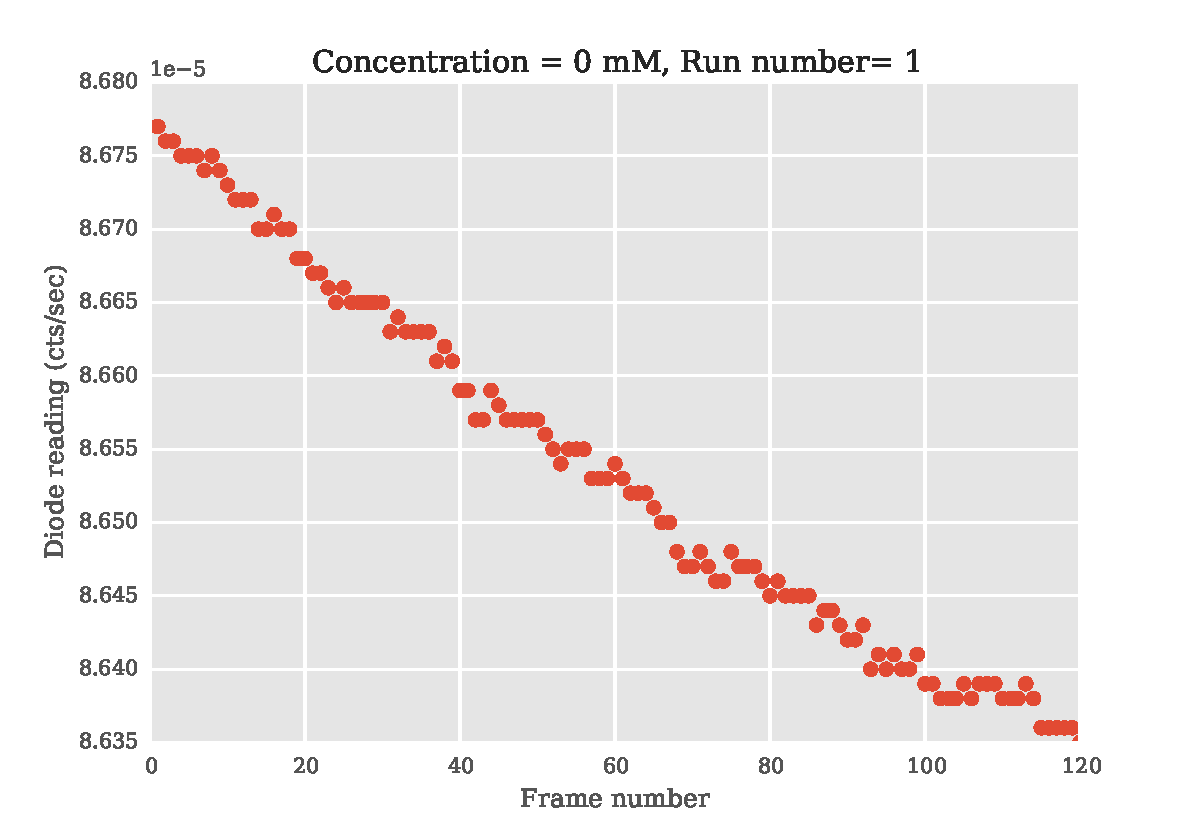
\includegraphics[width=\textwidth]{figures/saxs/np_diode_readings.pdf}
            \caption{}
            \label{fig:Diode readings}
    \end{subfigure}
    \\
    \begin{subfigure}[b]{0.7\textwidth}
            \centering
            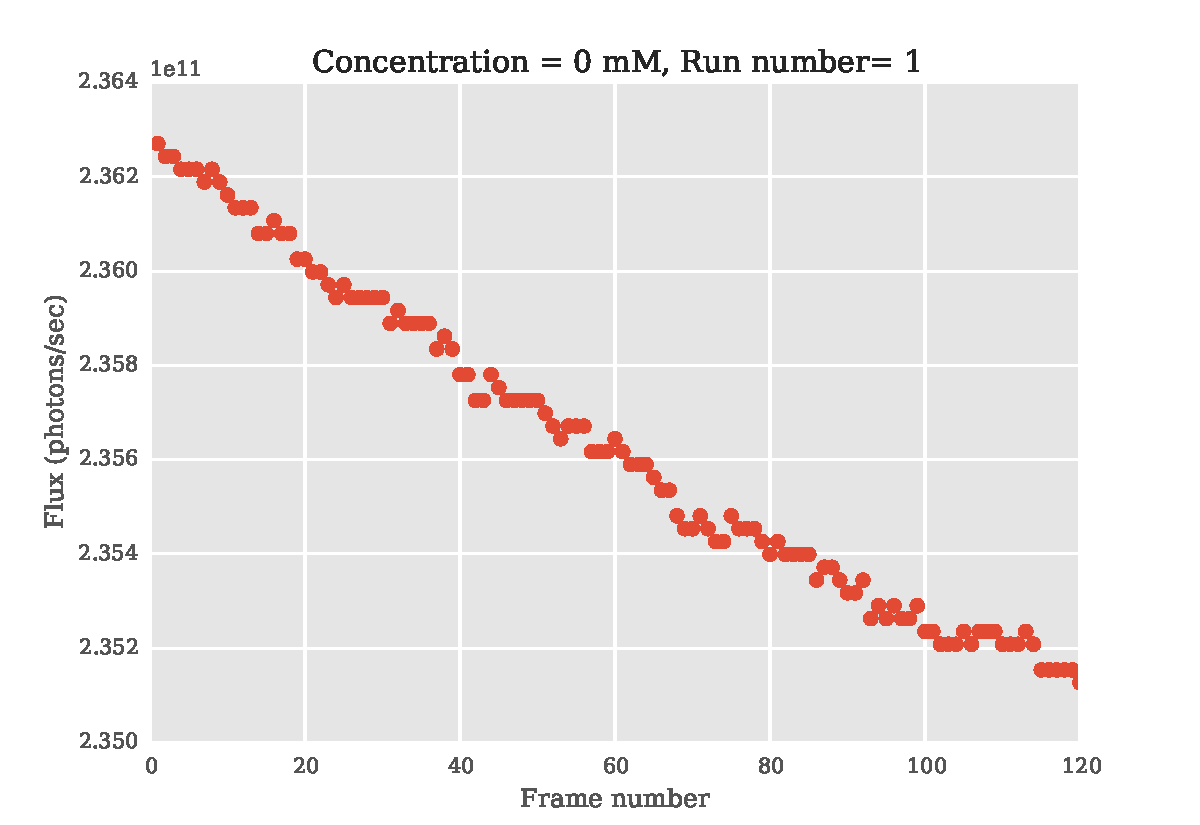
\includegraphics[width=\textwidth]{figures/saxs/np_flux_estimates.pdf}
            \caption{}
            \label{fig:Flux estimates}
    \end{subfigure}
    \caption{Diode readings and flux estimates during the first SAXS run for the GI sample with no additive (hence concentration = $0\ mM$). (a) It can clearly be seen that the diode readings decrease throughout the experiment. (b) As a result of the decreasing diode readings the corresponding flux decreases too.}
    \label{fig:Diode and flux readings}
\end{figure}
The 2-dimensional X-ray beam profile was determined from a mixture of measurements, spline interpolation and averaging.
A $100 \mu m$ diameter circular aperture was used to scan across the X-ray beam area and take measurements at $10 \mu m$ intervals.
These readings were then used to determine the entire beam profile using a mixture of the bivariate spline approximation and averaging as outlined in section \textcolor{red}{...(The method will be described in the previous chapter on beam the beam measurements)...}. The resulting beam is shown in Figure~\ref{fig:SAXS beam profile}.
\begin{figure}
    \centering
    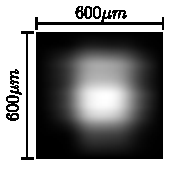
\includegraphics[width=0.5\textwidth]{figures/saxs/SAXS_beam.pdf}
    \caption{2-dimensional greyscale image of the beam used in the SAXS experiment. Multiple diode measurements were taken with a $100 \mu m$ diameter circular aperture as it scanned across the X-ray beam area. These readings were subsequently used to determine the entire beam profile using a mixture of the bivariate spline approximation and averaging as outlined in section \textcolor{red}{...(The method will be described in the previous chapter on beam the beam measurements)...}}
    \label{fig:SAXS beam profile}
\end{figure}

\textcolor{red}{
    \begin{myenumerate}
        \item \hypertarget{todo:Detector type}{\textbf{TODO:} Need to ask Adam round what the detector was along with frame rate and readout.}
    \end{myenumerate}
}
The data were recorded using a \textcolor{red}{...detector type...}.
\textcolor{red}{...$15\ \mu l$...} of each sample was loaded into a $1.8\ mm$ quartz capillary ($1.7\ mm$ internal diameter) held at room temperature.
For each additive, data were collected at each concentration (given in section \ref{sub:Sample preparation}), and each of these runs was repeated 3 times.
The exposure time for each frame was 1 second and a total of 120 frames were collected for a single run.
During each experimental run, the sample was kept static.
For each concentration a single run with only the buffer (no protein) was also taken so that a suitable buffer correction could be applied during data analysis.

\subsection{Dose calculation}
\label{sub:Dose calculation}
Dose calculations for both experiments were performed using RADDOSE-3D with the modifications described in section \ref{sec:Extending RADDOSE-3D for SAXS} for modelling SAXS experiments.

\subsubsection{Experiment 1}
\label{subs:Experiment 1 - dose calc}
An example input file for experiment 1 can be seen in Figure~\ref{fig:SAXS example input - Rebecca}. The beam profile was assumed Gaussian with full width at half maximum of $110\ \mu m \times 200\ \mu m$.
\begin{figure}
    \centering
    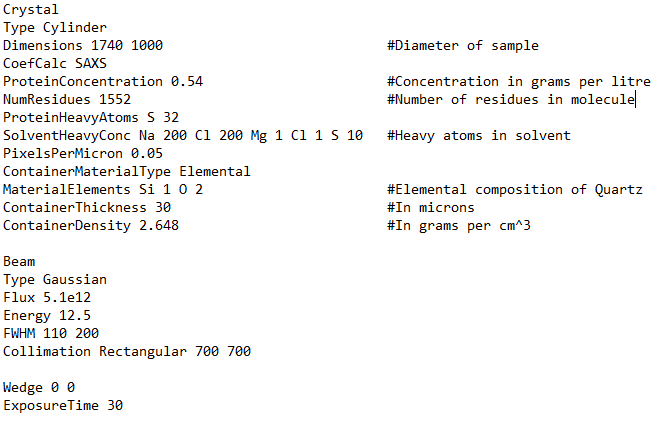
\includegraphics[width=0.5\textwidth]{figures/saxs/rebecca_raddose_input.png}
    \caption{RADDOSE-3D input file used for the dose calculations in experiment 1. \textcolor{red}{There is a discrepancy with the flux for the input file and the flux Rebecca reported in her dissertation (experiment 1). What should I do? (bear in mind there were a few other mistakes which wouldn't make sense if I kept them in so I changed some of them)}
    }
    \label{fig:SAXS example input - Rebecca}
\end{figure}

\subsubsection{Experiment 2}
\label{subs:Experiment 2 - dose calc}
The beam image shown in Figure~\ref{fig:SAXS beam profile} was read directly into RADDOSE-3D and the corresponding flux values recorded for each frame were used to ensure accurate dose estimates.
The FASTA sequence file used to determine the atomic composition was downloaded from \textcolor{red}{PDB entry 4US6}, a tetrameric form of GI.
The elemental composition of the quartz capillary was entered into RADDOSE-3D as $SiO_2$.
The capillary thickness was given as $50\ \mu m$ and a density of $2.648\ g/cm^3$ was used.
